% !TEX root = ./article.tex

\documentclass{article}

\usepackage{mystyle}
\usepackage{myvars}



%-----------------------------

\begin{document}

	\maketitle % Insert title

	\thispagestyle{firststyle}


%-----------------------------
%	ABSTRACT
%-----------------------------

	\begin{abstract}
		\noindent En este documento se realiza una descripción acerca del algoritmo de aprendizaje automático basado en \emph{máquinas de vectores soporte (SVM)}. Además, se resuelve de manera gráfica la tarea de aprendizaje mediante SVM sobre un conjunto de datos sencillo. Por último, se realizan distintos experimentos utilizando el conjunto de datos \emph{Wine} para tratar de encontrar la función kernel óptima sobre dicho conjunto de datos.
	\end{abstract}

%-----------------------------
%	TEXT
%-----------------------------


	\section{Introducción}
	\label{sec:introducción}

		\subsection{Máquinas de Vectores Soporte}
		\label{sec:support-vector-machine}

			\paragraph{}
			Las máquinas de vector soporte son una estrategia de aprendizaje similar a la regresión lineal. Sin embargo, añade la restricción de que el hiperplano de separación entre los conjuntos de datos a clasificar debe poseer la propiedad de ser el de mayor distancia entre los dos conjuntos de datos.

			\paragraph{}
			De esta manera, el clasificador obtenido será mucho más preciso ya que la solución generaliza mejor la diferencia entre clases por lo que se reduce en mayor medida el sobreajuste. El algoritmo funciona mediante el apoyo entre los puntos de clases distintas más cercanos entre si, a los cuales se denomina vectores soporte. La razón de ello es que si el plano se construye tratando de maximizar la distancia a estos puntos, el resultado es equivalente a si se quisiera maximizar sobre el conjunto de datos completo.

	\section{Experimento sobre conjunto de datos sencillo}
	\label{sec:e1}

		\paragraph{}
		En esta sección se describe de manera teórica cómo funcionaria la fase de aprendizaje sobre el conjunto de datos sencillo, el cual se muestra en la tabla \ref{table:e1_dataset}, utilizando el algoritmo de \emph{máquinas de vector soporte (SVM)}. Puesto que este algoritmo trata de maximizar la distancia del hiperplano de separación entre las dos clases teniendo en cuenta únicamente los puntos de clases distintas más cercanos entre sí los cuales se denominan vectores soporte, el resto de instancias no se tienen en cuenta para la construcción del hiperplano.

		\begin{table}
			\centering
			\begin{tabu}{ | c | c | c |}
				\hline
				\multicolumn{3}{ | c | }{Simple Dataset} \\ \hline
				\bfseries $x_1$ & \bfseries $x_2$ & \bfseries $d(x)$
				\csvreader[head to column names]{../datasets/simple.csv}{
					1=\one, 2=\two, 3=\three
				}
				{\\\hline\one&\two&\three}
				\\\hline
			\end{tabu}
			\caption{Conjunto de datos Simple}
			\label{table:e1_dataset}
		\end{table}

		\paragraph{}
		Para elegir el hiperplano óptimo por tanto hay que tratar de maximizar la distancia del mismo a las dos clases a clasificar. Puesto que en este caso se ha utilizado un kernel lineal, el hiperplano se puede representar como una recta sobre el espacio de dos dimensiones al cual pertenece el conjunto de datos. Para la construcción del mismo el algoritmo de máquinas de vector soporte se apoya en la utilización de dos rectas paralelas entre si en las cuales se apoyan los vectores soporte de cada conjunto de datos. El hiperplano a construir por tanto, se debe encontrar en el punto intermedio de estas, por lo que también es paralelo a ellas.

		\paragraph{}
		Esta construcción se puede apreciar en la figura \ref{fig:e1-plot} de manera visual. Tal y como se puede ver, no existe un otro hiperplano para el conjunto de datos utilizado que maximice en mayor medida la distancia entre el hiperplano y los vectores soporte de las dos clases.

		\begin{figure}
			\begin{center}
				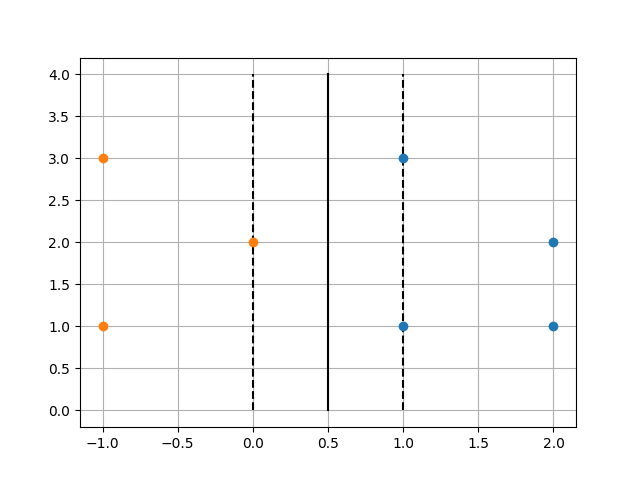
\includegraphics[width=\textwidth]{graph}
			\end{center}
			\caption{Representación gráfica del hiperplano construido a partir de máquinas de vector soporte SVM sobre el conjunto de datos simple}
			\label{fig:e1-plot}
		\end{figure}


	\section{Experimento sobre Wine Dataset}
	\label{sec:e2}

		\paragraph{}
		El conjunto de datos utilizado para los experimentos que se describirán en esta sección es \textbf{Wine Data Set} \cite{dataset:wine}, compuesto por \textbf{178 instancias}. Dichas instancias contienen \textbf{12 atributos} de carácter númerico. La \textbf{clase de destino es de carácter numérico}. Sin embargo, en este caso es de tipo entero, por lo que puede ser vista como una variable categórica. En cuanto a la metodología experimental, se ha seguido una extrategia de \textbf{HoldOut} con particionamiento de los datos de manera que $\frac{2}{3}$ son utilizados en la fase de entrenamiento y $\frac{1}{3}$ en la de test.

		\paragraph{}
		El experimento realizado consiste en la búsqueda de valores óptimos del kernel de las máquinas de vector soporte utilizadas. Se han utilizado kernels polinomiales (variando el grado máximo de 1 a 8) y kernels gaussianos. En el caso de los kernels lineales, los resultados se muestan en la tabla \ref{table:sol-e2-lin} de forma tabular y en la figura \ref{plot:sol-e2-lin} de manera gráfica. Tal y como se puede apreciar el óptimo se encuentra utilizando polinomios de grado 2 o 3. En este caso se preferiría el caso de polinomios de grado 2, lo cual reduce la complejidad del problema debido al número de valores a calcular.

		\csvreader[
		  longtable=| c | c |,
		  table head=\hline\bfseries \# Grado &\bfseries Tasa de Error \\\hline,
			table foot= \caption{Tasa de error obtenida al utilizar kernels lineales en la máquina de vectores soporte sobre el conjunto de datos \emph{Wine}}\label{table:sol-e2-lin}\\,
		  late after line=\\\hline,
		  before reading={\catcode`\#=12},after reading={\catcode`\#=6}
		]{../results/results.csv}{1=\k,2=\error}{\k & \error}

		\paragraph{}
		En el caso de las funciones gaussianas, la tasa de error encontrada se muestra en la tabla \ref{table:e3}. En este caso tan solo se ha incluido un valor debido a que a pesar de probar con distintos valores para el exponente, el resultado obtenido no varía, por tanto se ha preferido no incluir los resultados de manera individual.

		\begin{figure}
			\begin{center}
				\begin{tikzpicture}
					\begin{axis}[
						% only scale the axis, not the axis including the ticks and labels
						scale only axis=true,
						% set `width' and `height' to the desired values
						width=0.9\textwidth,
						height=0.3\textwidth,
						]
						\addplot table [x=k, y=error, col sep=comma] {../results/results.csv};
					\end{axis}
				\end{tikzpicture}
			\end{center}
			\caption{Tasa de error obtenida al utilizar kernels lineales en la máquina de vectores soporte sobre el conjunto de datos \emph{Wine}}
			\label{plot:sol-e2-lin}
		\end{figure}


		\begin{table}
			\centering
			\small
			\begin{tabu}{ | c | c | }
				\hline
				\multicolumn{2}{ | c | }{SVM con kernel gaussiano} \\ \hline
				Datos & Tasa de Error \\ \hline
				Pruebae								& $0.016393$	\\
				\hline
			\end{tabu}
			\caption{Tasa de error obtenida al utilizar un kernel gaussiano en la máquina de vectores soporte sobre el conjunto de datos \emph{Wine}}
			\label{table:e3}
		\end{table}


%-----------------------------
%	Bibliographic references
%-----------------------------
	\nocite{subject:taa}
	\nocite{garciparedes:machine-learning-support-vector-machine}
	\nocite{dataset:wine}
	\nocite{tool:weka}
  \bibliographystyle{alpha}
  \bibliography{bib/bib}

\end{document}
